\documentclass[conference]{IEEEtran}
\IEEEoverridecommandlockouts
% The preceding line is only needed to identify funding in the first footnote. If that is unneeded, please comment it out.
\usepackage{cite}
\usepackage{amsmath,amssymb,amsfonts}
\usepackage{algorithmic}
\usepackage{graphicx}
\usepackage{textcomp}
\usepackage{xcolor}
\usepackage{url}
\usepackage[hidelinks]{hyperref}
\usepackage{booktabs}
\usepackage{tabularx}
\usepackage{booktabs}
\usepackage{csvsimple}
\usepackage{tikz}
\usepackage{pgfplots}
\usepackage{adjustbox}
\usepackage{placeins}
\pgfplotsset{compat=1.18}

\def\BibTeX{{\rm B\kern-.05em{\sc i\kern-.025em b}\kern-.08em
    T\kern-.1667em\lower.7ex\hbox{E}\kern-.125emX}}
\begin{document}


\title{Evaluating the Security Posture of Canadian Government Authority Websites\\
\thanks{This work was supported by the CSA Group Undergraduate Research Scholarship.}
}


\author{\IEEEauthorblockN{1\textsuperscript{st} Isaac Latta}
\IEEEauthorblockA{\textit{Department of Engineering} \\
\textit{Thompson Rivers University}\\
Kamloops, BC, Canada \\
lattai11@mytru.ca}
\and
\IEEEauthorblockN{2\textsuperscript{nd} Sina Keshvadi}
\IEEEauthorblockA{\textit{Department of Engineering} \\
\textit{Thompson Rivers University}\\
Kamloops, BC, Canada \\
skeshvadi@tru.ca}
}

\maketitle

\begin{abstract}
  
  Public-sector web services are central to citizen-facing digital delivery and rely on implicit public trust, yet their security posture is rarely benchmarked beyond basic HTTPS adoption. We present a comparative measurement study of public-sector web security configuration centered on Canadian government authority websites, and contextualize the results against Canadian critical sectors (finance, education, and energy) and government authorities in the United States and United Kingdom, covering 1{,}939 unique origins. 
  To enable consistent, standards-aligned evaluation, we operationalize Canadian Centre for Cyber Security (CCCS) guidance---augmented with OWASP/MDN recommendations and relevant RFCs---into a set of measurable benchmarks and assess transport security, browser-enforced controls, vulnerability disclosure readiness, and information leakage signals.
  
  Our findings show substantial implementation gaps in Canadian authorities: while HTTPS is common, only 59.73\% deploy HTTP Strict Transport Security (HSTS) and only 69.1\% negotiate TLS~1.3, lagging both international counterparts and the Canadian financial sector. We further observe that 47.2\% of authority origins exhibit technology leakage in error responses, and fewer than 2\% support standardized vulnerability disclosure via \texttt{security.txt}. Overall, the gaps we identify largely reflect inconsistent deployment of well-known, configuration-driven controls rather than a lack of technical feasibility.

\end{abstract}

\begin{IEEEkeywords}
Web Security, Government Websites, HTTPS, Security Headers, Vulnerability Disclosure
\end{IEEEkeywords}

% \section{Introduction}
% Government and public authority websites are widely trusted entry points for essential public services, ranging from information dissemination to online transactions. As these sites mediate high-trust interactions at population scale, weaknesses in their web security posture can translate into meaningful harm for users and can undermine confidence in digital government.

% Assessing ``web security posture'' is increasingly non-trivial. Modern web services are built from layered, interdependent components and deliver functionality through complex client--server interactions, third-party dependencies, and rapidly evolving browser behaviors~\cite{kumar2017security}. As a result, a narrow check (e.g., whether a site supports HTTPS) is insufficient to characterize practical exposure. Meaningful evaluation must account for transport-layer protections (encryption, downgrade resistance, and protocol configuration) alongside browser-enforced controls (security headers and cookie attributes) that shape what the user agent will permit at runtime~\cite{owasp_http_security_response_headers,mdn_secure_cookie_configuration}.

% Canada presents a particularly important context for measurement because best practices are primarily communicated through guidance rather than uniformly enforceable directives. The Canadian Centre for Cyber Security (CCCS) publishes recommendations spanning securely configured protocols and website security considerations~\cite{cccs-itsp-40062,cccs-itsm-60005}. By contrast, peer jurisdictions have operationalized web-security expectations through more prescriptive federal policy instruments. For example, U.S.\ federal web services are guided by OMB M-15-13 and supporting HTTPS compliance guidance~\cite{omb-m-15-13,uscio-https-guide}, and binding operational directives have been used to mandate specific cybersecurity actions across agencies~\cite{cisa_bod_18_01}. In the UK, central government guidance for digital services specifies HTTPS-only deployment and explicitly calls for HSTS~\cite{uk-using-https-service-manual}. These differing governance models motivate a practical question: to what extent are modern, recommended web security controls consistently adopted across Canadian authority websites, and where do measurable gaps persist?

% Several control classes are especially relevant to this question. At the transport layer, HTTPS reachability and HTTPS-only enforcement are foundational, and HSTS (RFC~6797) strengthens downgrade resistance by instructing user agents to automatically upgrade future requests to HTTPS~\cite{rfc6797}. Beyond enforcement, protocol versioning matters: TLS~1.3 (RFC~8446) is the modern standard~\cite{rfc8446}, while TLS~1.0 and TLS~1.1 are formally deprecated~\cite{rfc8996} and are discouraged by widely cited government and standards guidance~\cite{nist_800_52r2,nsa_eliminating_obsolete_tls}. At the application layer, security response headers and cookie attributes provide browser-enforced constraints that reduce exposure to common web attack classes (e.g., framing abuse, content injection, and cross-site request risks)~\cite{owasp_http_security_response_headers,mdn_secure_cookie_configuration}. Finally, operational and hygiene controls matter for remediation and reconnaissance: standardized vulnerability disclosure via \texttt{security.txt} (RFC~9116) can lower the friction of reporting security issues~\cite{rfc9116,cisa_securitytxt_simple_file_big_value}, while verbose error handling and technology-revealing metadata can leak information helpful to attackers, including the exposure class captured by CWE-209~\cite{cwe_209,owasp_improper_error_handling}.

% In this work, we translate heterogeneous guidance into a practical measurement baseline by consolidating CCCS recommendations with widely used standards and best-practice references (e.g., OWASP, MDN, and relevant RFCs) into a concrete set of web security requirements~\cite{cccs-itsp-40062,cccs-itsm-60005,owasp_http_security_response_headers,mdn_secure_cookie_configuration,rfc6797,rfc8446,rfc9116}. Building on this baseline, we design and implement an automated web security scanner to measure security posture at scale. Our scanning pipeline (i) normalizes and resolves URLs to the final destinations that users actually reach, (ii) distinguishes \emph{origin-scoped} controls (e.g., HTTPS enforcement, HSTS, and TLS configuration) from \emph{endpoint-scoped} controls (e.g., security headers and cookie attributes) that may vary by path and response, and (iii) applies conservative, non-invasive safeguards suitable for ethical measurement of public-facing services. Where relevant, our approach is informed by established measurement and design-science methodology for building artifacts intended for systematic evaluation~\cite{peffers2007design}.

% A number of tools support point-in-time testing of individual facets of web security posture, including transport-layer scanners and header graders~\cite{tool_ssllabs_ssltest,tool_testsslsh,tool_mozilla_observatory,tool_securityheaders}. More comprehensive dynamic scanners can probe for vulnerabilities, but their primary objective is discovery rather than population-level benchmarking of control adoption~\cite{tool_owasp_zap}. Our emphasis is instead on a unified, standards-aligned posture assessment suitable for large-scale comparative measurement across many sites, with explicit separation of origin and endpoint scope.

% Our primary focus is Canadian government authority websites. To interpret the results in a broader context, we also apply the same methodology to selected Canadian critical sectors and to peer government authority populations in the United States and United Kingdom, enabling benchmarking against jurisdictions with more prescriptive web-security policy~\cite{omb-m-15-13,uscio-https-guide,uk-using-https-service-manual}. Accordingly, this work addresses the following research questions: (i) how does adoption of transport protections (HTTPS reachability, HTTPS-only enforcement, HSTS, and modern TLS) vary across Canadian authorities and benchmark populations~\cite{rfc6797,rfc8446,cccs-itsp-40062}; (ii) how widely are browser-enforced controls deployed at final endpoints~\cite{owasp_http_security_response_headers,mdn_secure_cookie_configuration}; (iii) how prevalent is standardized vulnerability disclosure~\cite{rfc9116,cisa_securitytxt_simple_file_big_value}; and (iv) how common is inadvertent information disclosure through response metadata and error handling~\cite{cwe_209,owasp_improper_error_handling}.

% The remainder of the paper is organized as follows. Section~II provides background and motivation, Section~III reviews related work, Section~IV describes datasets and methodology, Section~V presents results, and Section~VI discusses implications, limitations, and future directions.

% \section{Background and Motivation}\label{sec:background}
% At a global scale, encrypted transport is now the baseline expectation for modern browsing. Major browser vendors actively surface security indicators to users and increasingly encourage (or default to) HTTPS-first behaviors~\cite{chrome-always-https,firefox-https-only-mode,apple-http-warning}. At the ecosystem level, longitudinal measurements similarly show that a substantial share of web traffic is now delivered over HTTPS~\cite{GoogleTransparencyHTTPS}. However, HTTPS adoption alone does not guarantee secure deployment: configuration quality varies widely, and many sites continue to omit stronger enforcement mechanisms or ship inconsistent hardening controls~\cite{SSLPulse}.

% Transport protections are necessary but insufficient. Even when encryption is present, real-world compromise often occurs through mechanisms that do not require breaking cryptography. For example, large-scale telemetry shows that a significant fraction of authentication attempts observed on the public Internet involve compromised credentials, reinforcing that attackers frequently succeed through credential reuse and account takeover rather than defeating TLS~\cite{CloudflareRadarAppLayer}. This reality is especially relevant for public-sector services that handle sensitive personal data and identity-linked workflows: improving security posture requires a holistic view that extends beyond ``HTTPS enabled'' to include enforcement depth and browser-side defenses.

% A key motivation for measuring web security posture in Canada is that guidance alone does not ensure consistent implementation. In the United States, secure web deployment has been operationalized through federal policy, including OMB Memorandum M-15-13 and supporting compliance guidance that establishes an HTTPS-only standard for federal websites and services~\cite{omb-m-15-13,uscio-https-guide}. The U.S.\ Cybersecurity and Infrastructure Security Agency (CISA) additionally issues Binding Operational Directives (BODs) that mandate specific cybersecurity actions for federal agencies, including directives relevant to web security practices~\cite{cisa_bod_18_01}. In the United Kingdom, central government guidance for digital services similarly specifies HTTPS-only deployment and explicitly calls for HSTS as a browser-level enforcement control~\cite{uk-using-https-service-manual}. By contrast, Canadian best practices for web security are primarily communicated through technical and management guidance, such as the Canadian Centre for Cyber Security’s recommendations on secure protocol configuration and website security considerations~\cite{cccs-itsp-40062,cccs-itsm-60005}. This difference in enforcement motivates a measurement question: do Canadian authority websites exhibit uniform adoption of modern controls, or do observable gaps remain in practice?

% Beyond transport, several under-measured areas materially affect practical exposure. First, standardized vulnerability disclosure is an operational control that can shorten time-to-remediation when issues are discovered. The \texttt{security.txt} standard (RFC~9116) defines a machine-readable mechanism to advertise security contacts and disclosure policies~\cite{rfc9116}. Yet prior research suggests adoption is generally low across the web, which can hinder responsible notification even when vulnerabilities are identified~\cite{findlay2021securitytxt}. Second, application-layer misconfigurations and information disclosure can persist even on HTTPS-enabled sites. Improper error handling and verbose responses can leak sensitive or operationally useful information, including details about frameworks and backend components; such leakage is captured by common weakness definitions like CWE-209 and is widely discouraged in secure development guidance~\cite{cwe_209,owasp-improper-error-handling}. Finally, modern browser-side controls---such as security response headers and cookie attributes---provide defense-in-depth against common web threats by constraining framing, content execution, and cross-site request behavior~\cite{owasp_http_security_response_headers,mdn_secure_cookie_configuration}.

% Taken together, these factors argue for a standards-aligned, multi-layer measurement approach that evaluates not only whether protections exist, but whether they are deployed with sufficient depth and breadth to meet contemporary expectations. This motivates our requirements-driven scanner and our empirical evaluation of adoption across Canadian authority websites, with benchmarking context drawn from other sectors and jurisdictions.

% \section{Related Work}\label{sec:related}
% Our work sits at the intersection of (i) empirical assessments of public-sector websites, (ii) large-scale measurement of web security configuration and control adoption, and (iii) operational practices such as vulnerability disclosure and information leakage reduction. This section summarizes the most relevant prior work and clarifies the gap addressed by our requirements-driven, origin/endpoint-aware methodology.

% \subsection{Security posture studies of government and public-sector websites}
% A number of studies have evaluated government and public-sector websites, but differ in target jurisdiction, granularity, and the set of controls measured. Dunbar et al.\ surveyed U.S.-related domains with an emphasis on secure network protocol deployment, highlighting variability in transport protections across a large population~\cite{dunbar4240917survey}. In Europe, Schiavone et al.\ studied HTTPS adoption in Italian municipal websites using a regulation-derived framework, demonstrating that adoption patterns can vary by region and municipal characteristics~\cite{schiavone2024municipality2https}. Valdaserides Olofsson et al.\ presented an automated tool and applied it to Swedish authorities, finding uneven adoption of security headers even when baseline HTTPS was present~\cite{valdaserides2024automated}. Beyond configuration, Hsiao et al.\ examined \emph{cyber autonomy} of G7 government websites, reporting substantial reliance on externally hosted resources and limited self-development, which introduces additional supply-chain and governance considerations~\cite{hsiao2019cyberautonomy}. Complementary public-sector evaluation work has also considered broader dimensions such as accessibility, usability, and security together, reinforcing that misconfigurations and exposure can persist across multiple quality attributes~\cite{csontos2021accessibility}.

% While these studies provide important evidence that public-sector web security is uneven, there remains limited Canada-focused benchmarking at population scale that simultaneously captures transport configuration, browser-enforced controls, standardized disclosure practices, and information leakage signals within a unified measurement framework. Moreover, prior work often reports site-level indicators without explicitly separating origin-scoped controls from endpoint-scoped behaviors that can change across final landing paths and redirect destinations~\cite{dunbar4240917survey,schiavone2024municipality2https,valdaserides2024automated}.

% \subsection{Large-scale web security measurement and scanning}
% The security measurement community has long developed techniques for Internet-scale and population-scale data collection. Felt et al.\ measured HTTPS adoption on the web and highlighted the practical measurement challenges that arise from redirects, mixed deployment, and heterogeneous configurations~\cite{felt2017measuring}. Internet-wide scanning platforms and methodologies have matured substantially over the past decade, enabling repeatable data collection across large target sets while emphasizing careful engineering and responsible scanning practices~\cite{durumeric2024ten}. These measurement foundations motivate our approach to URL normalization and redirect resolution prior to evaluating control adoption.

% In practice, many widely used tools provide deep, point-in-time testing of specific facets of web security posture. For transport-layer configuration, SSL Labs and \texttt{testssl.sh} offer detailed analysis of protocol versions and related weaknesses~\cite{tool_ssllabs_ssltest,tool_testsslsh}. For application-layer hardening, header graders such as Mozilla HTTP Observatory and SecurityHeaders.com summarize the presence of security-relevant HTTP headers and recommended mitigations~\cite{tool_mozilla_observatory,tool_securityheaders}. Dynamic application scanners such as OWASP ZAP can perform deeper web application testing, but their primary goal is vulnerability discovery rather than population-level measurement of control adoption~\cite{tool_owasp_zap}. Consequently, while these tools are valuable for auditing individual sites, they are not typically designed as an integrated, standards-aligned methodology for benchmarking large sets of public-sector websites.

% \subsection{Vulnerability disclosure and information leakage}
% Standardized vulnerability disclosure mechanisms can reduce friction for coordinated reporting and remediation. The \texttt{security.txt} standard (RFC~9116) defines a machine-readable format to advertise security contacts and disclosure-related metadata~\cite{rfc9116}. CISA has also encouraged adoption of \texttt{security.txt} as a practical step that improves vulnerability notification pathways~\cite{cisa_securitytxt_simple_file_big_value}. However, adoption remains limited at Internet scale; Findlay and Abdou characterized \texttt{security.txt} deployment and demonstrated that even when present, completeness and usage vary significantly~\cite{findlay2021securitytxt}. Further, coordinated disclosure can be operationally complex; recent work highlights real-world challenges that organizations face when implementing disclosure processes and responding to reports~\cite{chen2024you}. These findings motivate measuring not only technical controls, but also whether basic disclosure affordances exist across public-sector populations.

% Information leakage through error handling and response metadata is another recurring class of exposure. OWASP guidance explicitly discourages improper error handling and overly verbose responses~\cite{owasp_improper_error_handling,owasp_error_handling}, and MITRE’s CWE taxonomy identifies information exposure through error messages (CWE-209) as a common weakness pattern~\cite{cwe_209}. Additionally, OWASP’s Top~10 has repeatedly emphasized security misconfiguration as a broad driver of real-world risk, which includes accidental disclosures and missing hardening controls~\cite{owasp_top10_a05_2021}. Together, this prior work supports including both disclosure mechanisms and information-leakage indicators as first-class measurement targets in posture assessments.

% \subsection{Summary of gaps and positioning of this work}
% Prior literature establishes that public-sector websites often exhibit uneven security posture and that tooling exists to test individual properties in depth. However, gaps remain for Canada-focused, standards-aligned benchmarking that: (i) consolidates Canadian guidance with widely adopted best practices into a single testable requirements baseline~\cite{cccs-itsp-40062,cccs-itsm-60005}; (ii) measures both transport-layer and browser-enforced controls within one methodology~\cite{owasp_http_security_response_headers,mdn_secure_cookie_configuration}; (iii) explicitly distinguishes origin-scoped controls (e.g., HTTPS enforcement, HSTS, TLS) from endpoint-scoped behaviors (e.g., headers/cookies on final landing pages) to reflect what users experience after redirects~\cite{felt2017measuring}; and (iv) incorporates operational controls and exposure signals such as \texttt{security.txt} and error/metadata leakage~\cite{rfc9116,cwe_209,owasp_improper_error_handling}. Our work addresses these gaps by providing a unified scanner and measurement framework and applying it to Canadian authority websites, with benchmarking context drawn from selected Canadian sectors and peer authority populations.

% \section{Methodology}\label{sec:methodology}
% This section describes (i) how target websites were selected, (ii) how URLs were normalized and resolved to obtain consistent measurement targets, (iii) the security requirements and tests implemented by our scanner, and (iv) safeguards and validation procedures used to support ethical, non-invasive measurement.

% \subsection{Website Selection and Data Sources}\label{subsec:sources}
% Websites were sourced from authoritative public registries and official directories to minimize inclusion bias and reduce reliance on ad hoc discovery. Canadian authority targets were compiled primarily from Government of Canada directories of federal departments and institutions~\cite{canada_depts,canada_institutions}, supplemented by additional official listings (e.g., Crown corporations and sector-specific authorities) where applicable. For Canadian benchmark sectors, we constructed datasets from authoritative lists such as the Canadian Bankers Association membership directory for banks~\cite{cba_member_banks_2024}, Universities Canada for post-secondary institutions~\cite{ca_unis_list}, and Electricity Canada for electricity providers~\cite{electric_canada_members}, with additional federally regulated infrastructure lists (e.g., pipelines and nuclear facilities) where relevant~\cite{cer_pipeline_companies,cnsc_nuclear_facilities}.

% For cross-jurisdiction authority benchmarking, U.S.\ authority targets were derived from the federal agency index~\cite{usa-agency-index}. UK authority targets were constructed using official UK Government Digital Service listings via the Collections API documentation~\cite{uk-gov-collections-api-docs}. In all datasets, each entry consisted of a candidate URL (or domain) intended to represent the public-facing web presence of the organization.

% \subsection{Key Definitions: Origins and Endpoints}\label{subsec:definitions}
% Because different classes of controls operate at different scopes, we distinguish between \emph{origins} and \emph{endpoints}. An \emph{origin} is defined by scheme, host, and port (e.g., \texttt{https://example.gov:443}), while an \emph{endpoint} is an origin plus a specific path (e.g., \texttt{https://example.gov/services/apply}). This distinction is important: transport-layer properties (e.g., TLS configuration and HSTS) are naturally origin-scoped, while browser-enforced controls such as security headers and cookie attributes can vary by endpoint and even by response type~\cite{felt2017measuring,owasp_http_security_response_headers}.

% \subsection{URL Normalization and Redirect Resolution}\label{subsec:normalization}
% To ensure consistent measurement and avoid duplicate counting, all candidate URLs were normalized to a canonical form prior to scanning. Hostnames were lowercased, default ports (80/443) were removed, and inputs without an explicit scheme were assigned a default scheme of HTTPS. Each normalized URL was then resolved by following HTTP redirects up to a fixed maximum depth, recording the chain of intermediate responses and the final destination. Redirect resolution is essential for measuring what end users actually experience, as many public-sector domains consolidate to shared platforms, CDNs, or canonical hostnames~\cite{felt2017measuring}.

% After resolution, we derive two target sets:
% \begin{itemize}
%   \item A set of unique \emph{origins} extracted from both entry and final destinations, used for origin-scoped tests (e.g., HTTPS reachability, HSTS, TLS probing).
%   \item A set of final \emph{endpoints} (final resolved URLs), used for endpoint-scoped tests (e.g., security headers and cookie attributes).
% \end{itemize}
% All endpoint-scoped measurements are performed on the final resolved endpoint only, since this is the URL a typical user agent interacts with after redirects.

% \subsection{Requirements Baseline and Test Suite}\label{subsec:tests}
% We translate guidance into a measurable baseline by consolidating Canadian recommendations from the Canadian Centre for Cyber Security (CCCS) with widely adopted standards and best-practice references (e.g., OWASP, MDN, and IETF RFCs). CCCS guidance motivates transport and web hardening expectations, including secure protocol configuration and website security considerations~\cite{cccs-itsp-40062,cccs-itsm-60005}. OWASP and MDN provide practical, implementable browser-side hardening recommendations, including security response headers and secure cookie configuration~\cite{owasp_http_security_response_headers,mdn_secure_cookie_configuration}. Standards references (RFCs) provide normative definitions for mechanisms such as HSTS and \texttt{security.txt}~\cite{rfc6797,rfc9116}. The resulting requirements baseline is operationalized through the following modules.

% \subsubsection{HTTPS Reachability, HTTPS-only Behavior, and HSTS}\label{subsubsec:https_hsts}
% For each origin, the scanner tests both HTTP and HTTPS reachability and whether HTTP access is upgraded to HTTPS via redirection. Where an origin is HTTPS-capable, the scanner evaluates HTTP Strict Transport Security (HSTS) as specified in RFC~6797 by checking for the \texttt{Strict-Transport-Security} header and parsing its directives~\cite{rfc6797}. We extract \texttt{max-age}, \texttt{includeSubDomains}, and \texttt{preload} signaling. In line with common deployment expectations, we additionally record whether HSTS is configured with a long-lived \texttt{max-age} sufficient for preload eligibility, as documented in browser and platform guidance~\cite{mdn_sts_header,chromium_hsts_preload}.

% \subsubsection{TLS Protocol Configuration}\label{subsubsec:tls}
% To profile each origin's TLS posture, the scanner performs constrained handshakes to determine which TLS protocol versions are supported. TLS~1.3 is treated as the modern baseline (RFC~8446)~\cite{rfc8446}, while TLS~1.0 and TLS~1.1 are considered deprecated (RFC~8996)~\cite{rfc8996}. CCCS guidance encourages prioritizing modern protocol versions and deprecating obsolete protocols~\cite{cccs-itsap-40016,cccs-itsp-40062}, consistent with widely cited directives such as NIST SP 800-52r2 and NSA guidance on eliminating obsolete TLS~\cite{nist_800_52r2,nsa_eliminating_obsolete_tls}. In addition to explicit protocol probes, the scanner performs a ``natural'' handshake using a modern client configuration to capture the negotiated protocol version representative of a typical user agent experience.

% \subsubsection{Standardized Vulnerability Disclosure (\texttt{security.txt})}\label{subsubsec:securitytxt}
% To assess vulnerability disclosure support, the scanner probes each origin for \texttt{security.txt} as specified in RFC~9116~\cite{rfc9116}. Requests are issued to both \texttt{/security.txt} and \texttt{/.well-known/security.txt}. A response is recorded as present when it returns \texttt{200 OK} and contains a minimally valid set of fields (e.g., a \texttt{Contact:} field and/or a syntactically valid \texttt{Expires:} date). We also record whether the \texttt{Expires} field is present and unexpired at measurement time. This module is motivated by the operational value of standardized disclosure channels and prior evidence that adoption is limited on the public web~\cite{cisa_securitytxt_simple_file_big_value,findlay2021securitytxt}.

% \subsubsection{Browser-enforced Security Headers and Cookie Attributes}\label{subsubsec:headers_cookies}
% For each final resolved endpoint, the scanner evaluates the presence of security response headers commonly recommended for modern web hardening. This includes controls that govern referrer leakage, framing, content execution, MIME sniffing, and feature access policy~\cite{owasp_http_security_response_headers,mdn_referrer_policy_config,chrome_permissions_policy,owasp_clickjacking_defense,owasp_csp_cheatsheet}. Where cookies are present, the scanner parses cookie attributes aligned with modern secure configuration guidance, including \texttt{Secure}, \texttt{HttpOnly}, and \texttt{SameSite}~\cite{mdn_secure_cookie_configuration,owasp_session_management_cookies}. These tests are endpoint-scoped because policies and cookie attributes can vary by path and response.

% \subsubsection{Information Leakage via Response Metadata and Error Handling}\label{subsubsec:leakage}
% To evaluate inadvertent information disclosure, we check (i) response headers that reveal server technologies and frameworks and (ii) verbosity of error handling. OWASP guidance discourages exposing technology-identifying metadata and emphasizes reducing disclosure through misconfiguration~\cite{owasp_secure_headers_project,owasp_top10_a05_2021}. For error handling, the scanner requests a deliberately non-existent path on each origin and analyzes the resulting response for signatures of technology disclosure and stack traces, reflecting exposure patterns captured by CWE-209 and related error-handling guidance~\cite{cwe_209,owasp_improper_error_handling,owasp_wstg_error_handling}. Signature construction is informed by commonly deployed web platforms and frameworks; to ground coverage in contemporary practice, we reference widely used developer ecosystem summaries when selecting representative technology classes~\cite{stackoverflow_survey_2025}.

% \subsection{Ethical Scanning Safeguards}\label{subsec:ethics}
% All measurements are performed using standard HTTP(S) requests and TLS handshakes only; the scanner does not inject exploit payloads and does not attempt authentication or state-changing operations. To reduce load on public services and avoid disrupting availability, the scanner enforces conservative timeouts, bounded redirect resolution, global and per-origin concurrency limits, and stop thresholds after repeated failures. This configuration is consistent with ethical measurement norms used in prior large-scale Internet measurement work, where minimizing risk and respecting operational constraints are primary design goals~\cite{durumeric2024ten}.

% \subsection{Implementation Validation}\label{subsec:validation}
% We validated scanner behavior using controlled ground-truth endpoints prior to deployment. Unit tests covered URL parsing and normalization, redirect handling, HTTPS reachability classification, \texttt{security.txt} discovery, and header/cookie parsing using local endpoints configured with specific behaviors. TLS probing was tested against controlled HTTPS servers with intentionally varied protocol configurations to confirm correct separation of successful and failed handshakes relative to deprecation guidance~\cite{rfc8996,cccs-itsp-40062}. Information-leak detection was validated using a curated set of representative error pages and stack traces across common backend languages, alongside negative-control content to reduce false positives. Finally, end-to-end integration tests exercised the full pipeline against local targets emulating secure, partially configured, and misconfigured deployments.

% \section{Results}\label{sec:results}
% This section summarizes the empirical findings produced by our standards-aligned scanner across all constructed datasets. Results are reported at two scopes: \emph{origin-scoped} measurements (e.g., HTTPS enforcement, HSTS, and TLS posture) and \emph{endpoint-scoped} measurements (e.g., security headers and cookie attributes observed on the final resolved landing page). Where applicable, we reference the relevant standards for the measured controls, including HSTS (RFC~6797)~\cite{rfc6797}, TLS~1.3 (RFC~8446)~\cite{rfc8446}, and \texttt{security.txt} (RFC~9116)~\cite{rfc9116}.

% \subsection{URL Resolution Outcomes}\label{subsec:results_resolution}
% Before measuring security controls, all candidate URLs were normalized and resolved to their final destinations (Section~\ref{subsec:normalization}). Table~\ref{tab:redirect_summary} reports the resolution outcomes by dataset, including the number of input URIs, final de-duplicated URIs, and unique origins derived from both entry and final destinations. Across datasets, most inputs successfully resolved to an HTTP 2xx endpoint, though resolution rates varied by sector and jurisdiction. A notable consolidation effect was observed in UK authorities, where a large number of input URLs mapped to a small set of final origins, reflecting centralization behind shared platforms and canonical hostnames.

% \subsection{Transport Security: HTTPS Enforcement, HSTS, and TLS}\label{subsec:results_transport}
% \subsubsection{HTTPS reachability and HTTP$\rightarrow$HTTPS upgrades}
% Table~\ref{tab:https_connectivity} reports HTTP/HTTPS reachability and upgrade behavior for each dataset, computed over the set of resolved origins. Canadian authority origins show high but incomplete transport reachability: 76.00\% were HTTPS-reachable, and among HTTP-accessible services 90.06\% redirected users to HTTPS while 6.43\% remained accessible over HTTP without upgrade. In contrast, UK authority origins exhibited complete reachability at the final-origin level and uniformly upgraded HTTP requests to HTTPS.

% \subsubsection{HSTS adoption and configuration strength}
% HSTS strengthens HTTPS-only enforcement by instructing user agents to automatically upgrade future requests to HTTPS for a specified time window (RFC~6797)~\cite{rfc6797}. Table~\ref{tab:https_hsts_quality} summarizes HSTS deployment among HTTPS-capable origins, reporting overall presence as well as configuration strength. Among Canadian authorities, 59.73\% of HTTPS-reachable origins set HSTS. Of the origins that deployed HSTS, 46.29\% met our ``strong'' criteria (long-lived policy with \texttt{includeSubDomains}) and 27.43\% signaled preload eligibility, consistent with common browser preload expectations~\cite{mdn_sts_header,chromium_hsts_preload}. Across all datasets, HSTS presence and strength varied substantially even when HTTPS reachability was high.

% \subsubsection{TLS protocol support and negotiated versions}
% Table~\ref{tab:tls_summary} reports TLS version support and the protocol negotiated in a ``natural'' handshake intended to reflect typical user-agent behavior. Canadian authority origins negotiated TLS~1.3 in 69.1\% of successful handshakes, with the remainder negotiating TLS~1.2. Legacy protocol support (TLS~1.0 and TLS~1.1) was observed at non-zero rates across most datasets, despite formal deprecation of these protocols~\cite{rfc8996} and long-standing guidance encouraging migration to modern configurations~\cite{cccs-itsp-40062,nist_800_52r2,nsa_eliminating_obsolete_tls}. Figure~\ref{fig:tls_stacked_auth_fin} visualizes negotiated TLS versions for authority and finance datasets, highlighting that Canadian authorities negotiate TLS~1.3 less frequently than the U.S.\ and U.K.\ authority benchmarks.

% \subsection{Standardized Vulnerability Disclosure (\texttt{security.txt})}\label{subsec:results_securitytxt}
% Table~\ref{tab:securitytxt_summary} reports \texttt{security.txt} adoption and field completeness. Overall deployment of \texttt{security.txt} (RFC~9116)~\cite{rfc9116} was rare across all measured populations. Among Canadian authority origins, only 1.1\% (4 of 375) published a \texttt{security.txt} file. All four files contained \texttt{Contact} information and included \texttt{Expires} fields; however, only 25\% had unexpired \texttt{Expires} values at measurement time. U.S.\ authority origins exhibited higher adoption (3.5\%), and a larger fraction of those maintained valid expiration dates.

% \subsection{Browser-Enforced Controls: Security Headers and Cookies}\label{subsec:results_headers_cookies}
% \subsubsection{Security response headers}
% Table~\ref{tab:security_headers_presence} summarizes adoption of key security headers on final resolved endpoints. Across datasets, legacy hardening headers were generally more common than modern policy mechanisms. In Canadian authorities, adoption was higher for traditional controls (e.g., \texttt{X-Frame-Options} and \texttt{X-Content-Type-Options}) than for modern policy-based headers such as CSP \texttt{frame-ancestors} and \texttt{Permissions-Policy}, which are emphasized in current best-practice guidance~\cite{owasp_http_security_response_headers,owasp_csp_cheatsheet,chrome_permissions_policy,mdn_csp_guide}.

% \subsubsection{Cookie security attributes}
% Table~\ref{tab:cookie_security_flags} reports cookie attribute usage among endpoints that set cookies, and the fraction meeting our recommended/sufficient cookie profile derived from modern secure-cookie guidance~\cite{mdn_secure_cookie_configuration,owasp_session_management_cookies}. In Canadian authorities, 28.2\% of sites set cookies. Among cookie-setting sites, 63.5\% set the \texttt{Secure} attribute, 48.7\% set \texttt{HttpOnly}, and 15.7\% set \texttt{SameSite} $\ge$ \texttt{Lax}. Only 3.5\% of Canadian authority cookie-setting sites met the recommended/sufficient cookie configuration criteria, indicating substantial room for improvement in browser-enforced session protection.

% \subsection{Information Disclosure via Metadata and Error Handling}\label{subsec:results_leakage}
% \subsubsection{Technology-revealing response headers}
% Table~\ref{tab:revealing_headers_summary} reports the distribution of technology-revealing headers, including the share of origins that expose at least one such header. Technology-revealing metadata was pervasive across all datasets. For Canadian authorities, 94.4\% of origins exposed at least one technology-revealing header, with 10.8\% exposing three or more. These findings align with longstanding guidance to remove unnecessary banner and fingerprinting information from responses~\cite{owasp_secure_headers_project,owasp_top10_a05_2021}.

% \subsubsection{Leakage in error responses}
% Table~\ref{tab:error_leaks_summary} summarizes the prevalence of leaked technology information in error responses generated by requests to non-existent paths. In Canadian authorities, 47.2\% of origins exhibited technology leakage in error responses, and 10.7\% disclosed explicit version information. Such leakage is consistent with common weakness patterns described in CWE-209 and discouraged by secure error-handling guidance~\cite{cwe_209,owasp_improper_error_handling,owasp_wstg_error_handling}. Comparable leakage rates were observed across benchmark authority datasets, reinforcing that error-handling verbosity remains an ecosystem-wide concern even where baseline HTTPS is present.

% \subsection{Summary of Key Findings}\label{subsec:results_summary}
% Overall, the results show that baseline HTTPS is prevalent across the measured populations, but stronger controls and operational practices are inconsistently deployed. In Canadian authority websites, gaps are most pronounced in (i) HSTS adoption and configuration depth~\cite{rfc6797}, (ii) modern browser-enforced policies and cookie attributes~\cite{owasp_http_security_response_headers,mdn_secure_cookie_configuration}, (iii) standardized disclosure affordances via \texttt{security.txt}~\cite{rfc9116}, and (iv) reduction of technology disclosure through response metadata and error handling~\cite{cwe_209,owasp_improper_error_handling}. These findings motivate the discussion in Section~\ref{sec:discussion}, where we interpret implications and identify low-effort remediation opportunities.

% \section{Discussion}\label{sec:discussion}
% This study provides a standards-aligned view of how web security controls are deployed across Canadian government authority websites, with comparative context drawn from selected Canadian critical sectors and peer authority populations in the United States and United Kingdom. Rather than focusing on exploitability, our results characterize \emph{adoption} and \emph{deployment quality} of configuration-driven controls that materially influence user exposure. In this section, we interpret key findings and outline practical implications for Canadian authorities.

% \subsection{Transport security is prevalent, but enforcement depth remains uneven}\label{subsec:discussion_transport}
% Across datasets, baseline HTTPS is common, and many HTTP-accessible services upgrade users to HTTPS (Table~\ref{tab:https_connectivity}). However, for Canadian authorities the remaining fraction of services that still permit HTTP without upgrade represents a persistent downgrade and interception opportunity, particularly for first-visit scenarios where a user agent has not yet learned an HSTS policy. HSTS (RFC~6797) is designed to close this gap by instructing clients to automatically enforce HTTPS-only access for a specified duration~\cite{rfc6797}. Consistent with that role, the adoption and \emph{strength} of HSTS configuration (Table~\ref{tab:https_hsts_quality}) is more informative than HTTPS reachability alone: even when HSTS is present, short \texttt{max-age} values or the absence of \texttt{includeSubDomains} can leave meaningful downgrade paths open. Browser preload mechanisms and deployment guidance emphasize long-lived HSTS policies and include-subdomain coverage for robust enforcement~\cite{mdn_sts_header,chromium_hsts_preload}.

% TLS posture similarly reflects a ``mostly modern, but not uniform'' picture. TLS~1.3 is the contemporary protocol standard (RFC~8446)~\cite{rfc8446}, while TLS~1.0 and TLS~1.1 are formally deprecated (RFC~8996)~\cite{rfc8996}. Government and standards guidance encourages eliminating obsolete protocol versions and aligning deployments with modern configurations~\cite{cccs-itsp-40062,nist_800_52r2,nsa_eliminating_obsolete_tls}. In practice, our measurements show non-zero legacy support across multiple datasets (Table~\ref{tab:tls_summary}), indicating that deprecation guidance has not been uniformly operationalized. While advertising legacy support does not imply immediate compromise, it broadens the attack surface and can enable weaker negotiations for atypical clients. A straightforward remediation strategy for many sites is to disable deprecated protocol versions at the edge (load balancer, reverse proxy, or CDN), which is often operationally feasible without application changes.

% \subsection{Browser-enforced controls lag behind transport controls}\label{subsec:discussion_browser}
% A consistent finding across the results is that browser-side hardening is less uniformly deployed than transport-layer protections (Table~\ref{tab:security_headers_presence} and Table~\ref{tab:cookie_security_flags}). This gap matters because browser-enforced policies reduce exposure to common web attack classes by constraining risky behaviors that HTTPS alone does not address. Modern best practice guidance highlights response headers (e.g., CSP directives, referrer policy controls, and permissions policies) as defense-in-depth mechanisms that can be deployed incrementally~\cite{owasp_http_security_response_headers,owasp_csp_cheatsheet,mdn_csp_guide,chrome_permissions_policy}. The weaker adoption of modern policy-based headers (relative to legacy hardening headers) suggests that many deployments are not yet leveraging the controls available in current browser platforms.

% Cookie configuration results show an even sharper shortfall. Secure session protection depends on correct use of \texttt{Secure}, \texttt{HttpOnly}, and \texttt{SameSite} attributes, which are well documented in practical implementation guidance~\cite{mdn_secure_cookie_configuration,owasp_session_management_cookies}. The low share of cookie-setting sites meeting recommended/sufficient attribute profiles (Table~\ref{tab:cookie_security_flags}) suggests that many authorities are exposed to avoidable session theft and cross-site request risks. Importantly, these mitigations are typically configuration-driven at the framework, application gateway, or identity layer, and can often be improved without major application rewrites.

% \subsection{Vulnerability disclosure remains rare despite clear standardization}\label{subsec:discussion_disclosure}
% Standardized vulnerability disclosure is a low-friction mechanism for improving remediation pathways when issues are discovered. The \texttt{security.txt} standard (RFC~9116) specifies a machine-readable location and format for advertising security contacts and disclosure metadata~\cite{rfc9116}. Guidance from public-sector security stakeholders has emphasized its practicality and value~\cite{cisa_securitytxt_simple_file_big_value}. Yet our results show near-zero adoption across measured datasets (Table~\ref{tab:securitytxt_summary}), consistent with prior work that characterizes \texttt{security.txt} as uncommon and often incomplete even when present~\cite{findlay2021securitytxt}. For Canadian authorities, the combination of low adoption and expired \texttt{Expires} fields (when present) indicates that vulnerability reporting pathways are frequently absent or poorly maintained. Given the minimal implementation cost---a static text file and a monitored contact route---this represents an actionable opportunity for improving security responsiveness.

% \subsection{Information leakage remains a pervasive, low-effort reconnaissance aid}\label{subsec:discussion_leakage}
% Across all datasets, technology-revealing response headers are widespread (Table~\ref{tab:revealing_headers_summary}), and a substantial fraction of origins leak technology details in error responses (Table~\ref{tab:error_leaks_summary}). While such disclosures are not vulnerabilities by themselves, they reduce the cost of attacker reconnaissance and can support targeted exploitation against known-vulnerable stacks or misconfigured components. OWASP guidance explicitly discourages unnecessary identifying headers and emphasizes reducing misconfiguration-driven exposure~\cite{owasp_secure_headers_project,owasp_top10_a05_2021}. Similarly, error-message disclosure is a recognized weakness class (CWE-209) and is discouraged by secure error-handling guidance~\cite{cwe_209,owasp_improper_error_handling,owasp_wstg_error_handling}. In many cases, remediation is configuration-driven (e.g., suppressing banners, adjusting framework error modes, and ensuring generic error pages), and can be implemented at gateways or application frameworks with limited functional risk.

% \subsection{What benchmarking suggests about governance and operationalization}\label{subsec:discussion_benchmarking}
% Benchmarking against other Canadian sectors and peer authority populations helps separate ecosystem-wide issues from Canada-specific gaps. Some weaknesses (e.g., metadata leakage and error verbosity) appear broadly prevalent, suggesting that certain misconfiguration patterns remain common across the modern web. Other gaps (e.g., lower frequency of TLS~1.3 negotiation for Canadian authorities in our datasets) suggest that operational maturity and modernization cadence may differ by organizational environment. These differences are plausibly influenced by governance and enforcement: Canadian authorities rely primarily on CCCS guidance~\cite{cccs-itsp-40062,cccs-itsm-60005}, while U.S.\ and U.K.\ public-sector practices are shaped by more prescriptive policy instruments and service guidance~\cite{omb-m-15-13,uscio-https-guide,cisa_bod_18_01,uk-using-https-service-manual}. While our study does not establish causality, the benchmarking results are consistent with the broader hypothesis that enforceable directives can accelerate and standardize adoption of baseline controls.

% \subsection{Practical remediation: configuration-first improvements}\label{subsec:discussion_remediation}
% A salient implication of our findings is that many of the measured gaps involve controls that are comparatively low-effort and configuration-driven. For example, disabling deprecated TLS versions and prioritizing modern configurations aligns with standards and widely cited guidance~\cite{rfc8996,cccs-itsp-40062,nist_800_52r2}. Enabling HSTS with a long-lived policy and appropriate scope is a well-defined mechanism with clear browser behavior~\cite{rfc6797,mdn_sts_header}. Deploying modern security headers and strengthening cookie attributes is supported by mature best-practice documentation and can often be rolled out incrementally with monitoring for compatibility regressions~\cite{owasp_http_security_response_headers,mdn_secure_cookie_configuration}. Publishing \texttt{security.txt} offers a lightweight, standardized disclosure channel~\cite{rfc9116,cisa_securitytxt_simple_file_big_value}. Finally, removing unnecessary technology banners and reducing error verbosity mitigates avoidable reconnaissance value~\cite{owasp_secure_headers_project,cwe_209}. Taken together, these controls represent practical steps that Canadian authorities can implement to better match the security expectations that accompany public trust in online services.

% \section{Conclusion}\label{sec:conclusion}
% This paper presented a standards-aligned, requirements-driven measurement of web security posture for Canadian government authority websites. We consolidated Canadian guidance from the Canadian Centre for Cyber Security (CCCS) with widely adopted standards and best practices (e.g., IETF RFCs, OWASP, and MDN) to define a practical set of measurable security requirements spanning transport protections, browser-enforced controls, standardized vulnerability disclosure, and indicators of inadvertent information disclosure~\cite{cccs-itsp-40062,cccs-itsm-60005,rfc6797,rfc8446,rfc9116,owasp_http_security_response_headers,mdn_secure_cookie_configuration,cwe_209}.

% Using an automated scanner that distinguishes origin-scoped controls from endpoint-scoped controls, we found that baseline transport encryption is prevalent across measured populations, but deployment depth and consistency remain uneven for Canadian authorities. In particular, stronger enforcement mechanisms (e.g., robust HSTS configuration) and modernization signals (e.g., default negotiation of TLS~1.3 and elimination of deprecated protocol versions) are not uniformly operationalized despite clear guidance and formal deprecation of legacy protocols~\cite{rfc6797,rfc8446,rfc8996,cccs-itsp-40062,nist_800_52r2,nsa_eliminating_obsolete_tls}. At the application layer, adoption of modern browser-enforced policies and secure cookie attributes lags behind transport protections, indicating that many authority endpoints are not yet leveraging mature, configuration-driven defenses documented in contemporary best-practice guidance~\cite{owasp_http_security_response_headers,mdn_secure_cookie_configuration,owasp_session_management_cookies}.

% Operational controls and hygiene signals further highlight actionable gaps. Standardized vulnerability disclosure via \texttt{security.txt} (RFC~9116) was rare, even though it is inexpensive to deploy and is explicitly promoted as a practical improvement to reporting pathways~\cite{rfc9116,cisa_securitytxt_simple_file_big_value}. In parallel, information disclosure through response metadata and verbose error handling remained common, which can lower the cost of attacker reconnaissance and is discouraged by established guidance and common weakness definitions~\cite{owasp_secure_headers_project,owasp_improper_error_handling,cwe_209}. Taken together, our findings suggest that many opportunities to strengthen the security posture of Canadian authority websites are configuration-first and can often be deployed at the edge (e.g., CDN/WAF/reverse proxy) without major application rewrites, improving alignment with existing Canadian recommendations and widely adopted international practice~\cite{cccs-itsp-40062,cccs-itsm-60005}.

% \subsection{Limitations}\label{subsec:limitations}
% This measurement study has several limitations. First, results reflect the scanner’s network vantage point and conservative ethical scanning configuration; some ``unreachable'' outcomes may reflect bot mitigation or WAF policies rather than true service unavailability. Second, endpoint-scoped measurements (headers and cookies) were collected from final landing-page responses; some services may apply stricter controls only on authenticated or high-value transactional paths~\cite{owasp_http_security_response_headers,mdn_secure_cookie_configuration}. Third, \texttt{security.txt} discovery was limited to the standard locations and did not follow cross-origin redirects, which may undercount organizations that centralize disclosure policy on separate domains~\cite{rfc9116}. Finally, this work evaluates adoption of security controls rather than exploitability: absence of a control indicates increased risk exposure, but does not necessarily imply the presence of a specific vulnerability~\cite{owasp_top10_a05_2021}.

% \subsection{Future Work}\label{subsec:futurework}
% Future work can extend this benchmarking methodology in several directions. First, longitudinal measurement would quantify change over time and enable evaluation of whether policy or operational interventions measurably improve posture. Second, expanding endpoint coverage beyond landing pages (e.g., authentication flows and other high-value workflows) would better capture how browser-enforced controls and cookie attributes vary across application surfaces~\cite{owasp_session_management_cookies,mdn_secure_cookie_configuration}. Third, deeper dependency and third-party resource analysis could quantify supply-chain exposure and autonomy properties in the Canadian public-sector web, complementing prior findings that government sites often rely on external infrastructure~\cite{hsiao2019cyberautonomy}. Finally, integrating richer TLS and header-quality scoring (beyond presence/absence) could more directly map observed configurations to concrete, standards-based compliance targets~\cite{cccs-itsp-40062,nist_800_52r2,owasp_http_security_response_headers}.

% \section*{Acknowledgments}
% We thank the anonymous reviewers for their constructive feedback. This work was supported in part by the Natural
% \bibliographystyle{IEEEtran}
% \bibliography{main}
% \end{document}
% % 

\section{Introduction}
  
  Government and public-sector websites increasingly deliver essential services online, and users often extend a high degree of trust to these domains. 
  Yet, modern web security depends on more than ``having HTTPS'': it also requires correct transport enforcement (e.g., HSTS), up-to-date TLS configurations, and browser-enforced controls that mitigate common web attacks. 
  While ecosystem-wide encryption has become the norm, configuration quality remains uneven across the web~\cite{GoogleTransparencyHTTPS,SSLPulse}. 
  This motivates a focused, evidence-based assessment of how well public-sector sites implement widely recommended security controls in practice.
  
  Canada presents an especially relevant case for benchmarking. 
  In the United States and United Kingdom, secure web deployment has been operationalized through enforceable policy and centralized guidance, including U.S.\ federal requirements for secure connections and operational directives for web security practices~\cite{omb-m-15-13,cisa_bod_18_01}, as well as UK service guidance emphasizing HTTPS-only deployment and HSTS~\cite{uk-using-https-service-manual}. 
  In contrast, Canadian best practices are primarily disseminated as technical and management guidance (e.g., on securely configuring network protocols and securing websites)~\cite{cccs-itsp-40062,cccs-itsm-60005}. 
  This difference in governance raises a practical question: do recommendations alone lead to consistent adoption of modern security controls across Canadian authorities?

  To answer this question, we conduct a large-scale, comparative measurement study of Canadian public-sector and critical-sector websites, using the U.S.\ and U.K.\ as reference points. 
  We develop an automated, non-invasive scanner that distinguishes \emph{origins} from \emph{endpoints} and evaluates: 
  (i) transport protections (HTTPS reachability, HTTP$\rightarrow$HTTPS enforcement, HSTS per RFC~6797, and negotiated TLS versions)~\cite{rfc6797}; 
  (ii) browser-enforced hardening (security response headers and cookie attributes)~\cite{owasp_http_security_response_headers}; 
  (iii) standardized vulnerability disclosure via \texttt{security.txt} (RFC~9116)~\cite{rfc9116}; and 
  (iv) inadvertent information disclosure through response metadata and error handling (e.g., CWE-209)~\cite{cwe_209}. 
  
  Our results show that baseline encryption is common but stronger controls are inconsistently deployed in Canadian authorities (e.g., HSTS and TLS~1.3 negotiation lag behind comparison jurisdictions), while vulnerability-disclosure signaling remains rare and technology leakage through headers and error responses is widespread. 
  % Collectively, these findings provide a data-driven baseline for prioritizing low-effort, configuration-based improvements that better align public-sector deployments with modern expectations.

\section{Background and Related Work}
  HTTPS is now the default expectation for modern web browsing, and the broader ecosystem has steadily shifted toward encrypted transport~\cite{GoogleTransparencyHTTPS}. 
  However, encryption alone does not ensure a secure deployment: many real-world failures stem from incomplete transport enforcement (e.g., missing HSTS), outdated TLS configurations, and inconsistent browser-side hardening~\cite{CloudflareRadarAppLayer}. 
  % Large longitudinal snapshots of popular sites show that configuration quality remains uneven even among widely visited domains (e.g., substantial fractions lacking strong HSTS deployment)~\cite{SSLPulse}. 
  Moreover, operational data suggest that most attacks succeed without breaking cryptography at all~\cite{CloudflareRadarAppLayer}. 
  % These trends motivate measuring not only whether encryption is present, but whether it is enforced and complemented by modern, defense-in-depth controls.
  
  % Canada is a particularly relevant case because governance differs from jurisdictions with enforceable web-security policy. In the United States, secure connections for federal web services have been mandated through policy (e.g., OMB M-15-13) and reinforced through operational directives and compliance guidance~\cite{omb-m-15-13,cisa_bod_18_01,uscio-https-guide}. 
  % The United Kingdom similarly provides central guidance for digital services that explicitly calls for HTTPS-only deployment and browser-enforced transport via HSTS~\cite{uk-using-https-service-manual}. 
  % By contrast, Canadian best practices for secure protocol configuration and website security are primarily disseminated as technical/management guidance (e.g., CCCS recommendations), without comparable enforcement mechanisms~\cite{cccs-itsp-40062,cccs-itsm-60005}.
  % This difference raises an empirical question: how consistently are modern controls adopted across Canadian public-sector sites, relative to peers with more directive governance?

  Prior research has measured government and public-sector web security, though scope and granularity vary. 
  Dunbar et al.\ surveyed U.S.-related domains using TLS/HSTS-centric indicators~\cite{dunbar4240917survey}. 
  Schiavone et al.\ assessed HTTPS usage across Italian municipalities using a framework aligned with regulatory expectations and examined regional differences~\cite{schiavone2024municipality2https}. 
  Valdaserides Olofsson et al.\ proposed an automated assessment tool for Swedish authorities and highlighted uneven adoption of HTTP security headers even where baseline HTTPS is present~\cite{valdaserides2024automated}. 
  % Complementary work by Hsiao et al.\ examined ``cyber autonomy'' of G7 government sites, showing extensive reliance on external resources and limited self-hosting, which can complicate consistent hardening~\cite{hsiao2019cyberautonomy}. 
  Collectively, these studies show that public-sector web posture can vary significantly across jurisdictions and that focusing solely on HTTPS presence can miss important configuration gaps.

  A parallel line of work and practice emphasizes tooling for configuration assessment. 
  Widely used scanners such as the Qualys SSL Labs Server Test and \texttt{testssl.sh} provide detailed analysis of TLS versions, ciphers, and common cryptographic weaknesses. At the application layer, graders such as Mozilla HTTP Observatory and SecurityHeaders.com summarize the presence of security-relevant HTTP response headers and recommended hardening controls~\cite{tool_mozilla_observatory}. Dynamic scanners such as OWASP ZAP can discover vulnerabilities via active testing, but they are not designed primarily for standards-driven, population-level benchmarking~\cite{tool_owasp_zap}. Finally, standardized vulnerability disclosure has been formalized by \texttt{security.txt} (RFC~9116), yet adoption has historically been low and remains an area of concern for vulnerability notification workflows~\cite{rfc9116}.

  % \subsection{Gaps addressed by this study}
  Despite prior work, several gaps remain. 
  First, Canada has not been the primary target population in comparable large-scale studies, and cross-jurisdiction comparisons that include Canada are limited~\cite{dunbar4240917survey,schiavone2024municipality2https}. 
  Second, many existing evaluations rely on coarse site-level indicators (e.g., HTTPS and HSTS presence) and do not consistently separate origin-scoped transport posture from endpoint-scoped browser controls~\cite{dunbar4240917survey,valdaserides2024automated}. 
  Third, vulnerability disclosure readiness and inadvertent information disclosure (e.g., through response headers and error handling) are often treated as secondary concerns despite their practical implications~\cite{rfc9116,cwe_209}. 

  To address these gaps, our study benchmarks Canadian public-sector and critical-sector sites against U.S.\ and U.K.\ peers using an automated, non-invasive scanner grounded in CCCS guidance and widely adopted standards (e.g., RFCs, OWASP, and MDN)~\cite{cccs-itsp-40062,cccs-itsm-60005,owasp_http_security_response_headers,mdn_sts_header}. 
  We measure 
  (i) transport protections (HTTPS reachability, HTTP$\rightarrow$HTTPS enforcement, HSTS, and negotiated TLS), 
  (ii) browser-enforced hardening at final endpoints (security headers and cookie attributes), 
  (iii) standardized vulnerability disclosure via \texttt{security.txt}, and 
  (iv) technology leakage via response metadata and error handling~\cite{rfc6797,rfc9116,owasp_secure_headers_project,cwe_209}.

% Methodology
\section{Methodology}
\label{sec:method}

\subsection{Website selection and datasets}
  We constructed datasets of public-sector \emph{authority} websites and critical-sector websites (education, finance, energy) for Canada, and comparable sets for the United States and United Kingdom. Sources were restricted to authoritative registries, official directories, and well-established sector lists (Table~\ref{tab:dataset_sources}). Each record contributes one or more candidate URLs that are later normalized and resolved before measurement.

\begin{table}[t]
 \caption{Overview of website datasets and primary data sources.}
 \label{tab:dataset_sources}
 \centering
 \scriptsize
 \setlength{\tabcolsep}{3pt}
 \renewcommand{\arraystretch}{1.15}
 \begin{tabularx}{\columnwidth}{l l X}
 \toprule
 Country & Sector & Primary data sources \\
 \midrule
 Canada & Authorities &
 Compiled from Government of Canada official directories of departments and federal institutions
~\cite{canada_depts,canada_institutions}; remaining provincial authority lists were obtained from
 official provincial directories. \\
 Canada & Finance &
 Schedule I and II banks from the Canadian Bankers Association~\cite{cba_member_banks_2024};
 credit unions from provincial regulator registries (manual consolidation). \\
 Canada & Education &
 Universities and Colleges from Universities Canada~\cite{ca_unis_list}. \\
 Canada & Energy &
 Electricity sector from Electricity Canada member list~\cite{electric_canada_members};
 oil/gas and nuclear from federal regulator registries~\cite{cer_pipeline_companies,cnsc_nuclear_facilities}. \\
 \addlinespace[0.4em]
 USA & Authorities &
 Federal agency index of U.S.\ government organizations~\cite{usa-agency-index}. \\
 USA & Finance &
 FDIC ``BankFind'' API~\cite{fdic-bankfind-api}; sampling by ten most populous states based on
 U.S.\ population statistics~\cite{us-population-stats}. \\
 USA & Education &
 U.S.\ Department of Education ``College Scorecard'' API~\cite{us-college-scorecard-docs};
 sampling by ten most populous states based on U.S.\ population statistics~\cite{us-population-stats}. \\
 USA & Energy &
 Edison Electric Institute list of member companies and their websites~\cite{edison-electric-member-sites}. \\
 \addlinespace[0.4em]
 UK & Authorities &
 GOV.UK Collections API (organization listings)~\cite{uk-gov-collections-api-docs}. \\
 UK & Finance &
 Bank of England PRA-regulated list~\cite{uk-pra-creditunions-list} cross-referenced against
 FCA developer resources~\cite{uk-fca-api-docs}. \\
 UK & Education &
 Discover Uni dataset of higher-education providers~\cite{hesa_discoveruni_2024}. \\
 UK & Energy &
 No dataset was constructed; we did not identify an authoritative, URL-complete registry of UK energy providers. \\
 \bottomrule
 \end{tabularx}
\end{table}


\subsection{Origin/endpoint model, normalization, and redirect}
  We distinguish between an \emph{origin} (scheme + host + port) and an \emph{endpoint} (origin + path). Origin-scoped measurements capture transport posture (e.g., TLS and HTTPS enforcement), while endpoint-scoped measurements capture browser-enforced controls (e.g., security headers and cookies) on the final landing page.

  All candidate URLs were canonicalized by lowercasing hostnames, removing default ports (80/443), and assigning \texttt{https://} to scheme-less entries. We then performed bounded redirect resolution using HTTP \texttt{GET} requests: non-3xx responses terminate resolution; 3xx responses are followed via \texttt{Location} header up to a maximum of eight hops. Chains exceeding the hop limit, or redirects without \texttt{Location}, are labeled as resolution errors. Each input URL is mapped to (i) its entry origin/endpoint and (ii) a single final resolved endpoint; origins are deduplicated across both sets before transport tests. Endpoint-scoped tests are executed only on the final resolved endpoint, reflecting what users ultimately load.

\subsection{Security posture tests}
  For each target, the scanner executes a suite of conservative, standards-aligned tests derived from CCCS guidance, RFCs, and widely used hardening recommendations (e.g., OWASP/MDN). Below we summarize the evaluated dimensions.

\subsubsection{HTTPS enforcement and HSTS}
  We assess 
  (i) HTTP and HTTPS reachability, 
  (ii) whether HTTP requests are upgraded to HTTPS via redirection, and 
  (iii) whether the origin deploys HTTP Strict Transport Security (HSTS) per RFC~6797~\cite{rfc6797}. 
  Canadian guidance recommends HTTPS-only deployment and secure protocol configuration~\cite{cccs-itsp-40062,cccs-itsm-60005}. When the \texttt{Strict-Transport-Security} header is present, we parse \texttt{max-age}, \texttt{includeSubDomains}, and \texttt{preload}. We treat preload eligibility as requiring \texttt{max-age} $\ge 31536000$ seconds and \texttt{includeSubDomains}, consistent with documented preload requirements~\cite{mdn_sts_header,chromium_hsts_preload}.

\subsubsection{TLS configuration}
  We profile supported TLS protocol versions and the version negotiated by a typical modern client. CCCS guidance prioritizes TLS~1.3 and recommends deprecating older protocols (TLS~1.0/1.1, SSL)~\cite{cccs-itsap-40016,cccs-itsp-40062}, consistent with broader guidance~\cite{nist_800_52r2,nsa_eliminating_obsolete_tls}. For each origin, the scanner attempts constrained handshakes for TLS~1.3, 1.2, 1.1, and 1.0 to record version support, and performs one ``natural'' handshake to record the negotiated version experienced in practice.

\subsubsection{Vulnerability disclosure via \texttt{security.txt}}
We check for RFC~9116 \texttt{security.txt} by probing both \texttt{/security.txt} and \texttt{/.well-known/security.txt}~\cite{rfc9116}. A file is considered present when the response returns \texttt{200 OK} and includes at least one \texttt{Contact:} field or a syntactically valid, future-dated \texttt{Expires:} field at scan time. We also record whether a canonical URL is provided.

\subsubsection{Security headers and cookie attributes (endpoint-scoped)}
On the final resolved endpoint, we evaluate browser-enforced security controls commonly recommended for modern deployments~\cite{owasp_http_security_response_headers,chrome_permissions_policy,gds_security_overview_websites}. Specifically, we detect presence of: \texttt{Referrer-Policy}, \texttt{X-Frame-Options}, \texttt{Content-Security-Policy} (and whether it includes \texttt{frame-ancestors}), \texttt{X-Content-Type-Options: nosniff}, and \texttt{Permissions-Policy}. For endpoints that set cookies, we parse \texttt{Secure}, \texttt{HttpOnly}, and \texttt{SameSite} attributes in line with common secure-cookie guidance~\cite{mdn_secure_cookie_configuration,cccs_itsp_40_111}.

\subsubsection{Information leakage via headers and error handling}
To quantify inadvertent disclosure, we check for technology-revealing response headers and version strings using OWASP-derived header
lists~\cite{owasp_secure_headers_project,owasp_secure_headers_remove_json}. 
We additionally request a single deliberately non-existent path of the form
\texttt{https://\textit{origin}/\_\_scanner\_404\_\_\textit{token}/}
(where \textit{token} is random per origin) and analyze textual error responses for framework banners, 
platform/database identifiers, and common stack-trace signatures. Ordinary HTTP status signaling alone (e.g., 404 or 500) was
 not classified as leakage. We treat disclosure through error messages as a relevant weakness class (e.g., CWE-209)~\cite{cwe_209}.

\subsection{Scanner implementation and validation}
To ensure ethical, non-invasive measurement, the scanner enforces conservative global and per-origin concurrency limits, short timeouts, and stop rules to avoid overloading targets. Authority sites were scanned with 15 global concurrent requests and 3 concurrent requests per origin; other sectors used 20 global and 5 per-origin concurrent requests. Requests used a 3\,s timeout; scanning stops after three HTTP failures or two TLS failures per origin. Measurements rely on standard HTTP(S) requests and TLS handshakes only; no exploit payloads are used.

We validated correctness using controlled ground truth prior to deployment. Unit tests covered URL parsing and normalization, redirect handling, HTTPS reachability, \texttt{security.txt} discovery, and header/cookie parsing using local endpoints with known behaviors. TLS probing was validated against local HTTPS servers configured to accept or reject specific protocol versions. Error-leak detection was tested against locally generated stack traces and error pages across common backend stacks, alongside negative controls to reduce false positives. Finally, end-to-end tests exercised all modules against a small suite of local servers representing secure, partially configured, and misconfigured targets.

% \begin{table}[t]
%   \caption{Overview of website datasets and primary data sources.}
%   \label{tab:dataset_sources}
%   \centering
%   \scriptsize
%   \setlength{\tabcolsep}{3pt}
%   \renewcommand{\arraystretch}{1.15}
%   \begin{tabularx}{\columnwidth}{l l X}
%   \toprule
%   Country & Sector & Primary data sources \\
%   \midrule
%   Canada & Authorities &
%   Compiled from Government of Canada official directories of departments and federal institutions
%  ~\cite{canada_depts,canada_institutions}; remaining provincial authority lists were obtained from
%   official provincial directories (manual lookup where no consolidated registry exists). \\
%   Canada & Finance &
%   Schedule I and II banks from the Canadian Bankers Association~\cite{cba_member_banks_2024};
%   credit unions from provincial regulator registries (manual consolidation). \\
%   Canada & Education &
%   Public-facing universities and colleges from Universities Canada~\cite{ca_unis_list}. \\
%   Canada & Energy &
%   Electricity sector from Electricity Canada member list~\cite{electric_canada_members};
%   oil/gas and nuclear from federal regulator registries~\cite{cer_pipeline_companies,cnsc_nuclear_facilities}. \\
%   \addlinespace[0.4em]
%   USA & Authorities &
%   Federal agency index of U.S. government organizations~\cite{usa-agency-index}. \\
%   USA & Finance &
%   FDIC ``BankFind'' API~\cite{fdic-bankfind-api}; sampling by ten most populous states based on
%   U.S.\ population statistics~\cite{us-population-stats}. \\
%   USA & Education &
%   U.S.\ Department of Education ``College Scorecard'' API~\cite{us-college-scorecard-docs};
%   sampling by ten most populous states based on U.S.\ population statistics~\cite{us-population-stats}. \\
%   USA & Energy &
%   Edison Electric Institute list of member companies and their websites~\cite{edison-electric-member-sites}. \\
%   \addlinespace[0.4em]
%   UK & Authorities &
%   GOV.UK Collections API (organization listings, filtered to ``live'')~\cite{uk-gov-collections-api-docs}. \\
%   UK & Finance &
%   Bank of England PRA-regulated banks list~\cite{uk-pra-creditunions-list} cross-referenced against
%   the FCA FSDeveloper API~\cite{uk-fca-api-docs}. \\
%   UK & Education &
%   Discover Uni dataset of higher-education providers~\cite{hesa_discoveruni_2024}. \\
%   UK & Energy &
%   No dataset was constructed; we did not identify an authoritative, URL-complete registry of UK energy providers. \\
%   \bottomrule
%   \end{tabularx}
% \end{table}

\section{Results}\label{sec:result}

We report results over the de-duplicated set of resolved origins and final landing endpoints produced by the normalization and redirect-resolution pipeline described in Section~\ref{sec:method}. 
% This section summarizes our findings after URL normalization and redirect resolution, followed by results for transport security, vulnerability disclosure, browser-enforced controls, and information leakage.
% Key outcomes are reported in Tables~\ref{tab:redirect_summary}--\ref{tab:error_leaks_summary} and Fig.~\ref{fig:tls_stacked_auth_fin}. 

% \subsection{URL \& origin normalization}
% Table~\ref{tab:redirect_summary} reports how input URLs map to measured endpoints. Across datasets, redirect resolution substantially reduced duplicates, producing a de-duplicated set of final URIs and unique origins used for analysis. 
% The UK Authorities dataset exhibited the strongest consolidation, with hundreds of input entries mapping to only four unique final origins after resolution. 
% Final successful (2xx) resolution rates varied by dataset, ranging from 68.4\% (CA Authorities) to above 90\% in most education, finance, and energy datasets. 

\subsection{Website security evaluation}

\subsubsection{Transport security}
Table~\ref{tab:https_connectivity} summarizes HTTP/HTTPS reachability and HTTP$\rightarrow$HTTPS upgrading behavior. Among Canadian authority origins, 76.00\% were HTTPS-reachable; among HTTP-accessible origins, 90.06\% redirected to HTTPS while 6.43\% remained available over HTTP without upgrade. 
In contrast, UK Authorities showed complete reachability at the final-origin level and universally redirected HTTP to HTTPS.

% table for https connectivity
  \begin{table}[t]
  \caption{HTTP/HTTPS connectivity outcomes by dataset (percent of origins).}
  \label{tab:https_connectivity}
  \centering
  \scriptsize
  \setlength{\tabcolsep}{3pt}
  \renewcommand{\arraystretch}{1.15}
  
  \begin{adjustbox}{max width=\columnwidth}
  % \resizebox{\columnwidth}{!}{%
  \csvreader[
  tabular=lrrrrrr,
  table head=\toprule
  Dataset &
  $n$ origins &
  HTTPS ok (\%)&
  HTTPS unreach. (\%)&
  HTTP ok (\%)&
  HTTP$\to$HTTPS (\%)&
  HTTP no redir. (\%) \\\midrule,
  late after line=\\,
  late after last line=\\\bottomrule
  ]{../results/comparison/https_hsts/https_hsts_enforcement_summary.csv}{%
  dataset_label=\Dataset,
  n_origins=\Norigins,
  pct_https_success=\PHttpsOk,
  pct_https_unreachable=\PUnreach,
  pct_http_probe_ok=\PHttpOk,
  pct_http_redirect_to_https=\PRedir,
  pct_http_no_redirect=\PNoRedir
  }{%
  \Dataset &
  \Norigins &
  \PHttpsOk &
  \PUnreach &
  \PHttpOk &
  \PRedir &
  \PNoRedir
  }%
  \end{adjustbox}
  \end{table}

Table~\ref{tab:https_hsts_quality} reports HSTS deployment among HTTPS-reachable origins. For Canadian authorities, 59.73\% of HTTPS-capable origins set HSTS; among those, 46.29\% met our ``strong'' criterion (one-year \texttt{max-age} with \texttt{includeSubDomains}) and 27.43\% indicated preload eligibility. 
Overall, HSTS presence and strength varied widely across jurisdictions and sectors, even when HTTPS reachability was high.

% table for hsts quality
\begin{table}[t]
  \caption{HSTS adoption and strength among HTTPS-capable origins (percent of HTTPS-ok).}
  \label{tab:https_hsts_quality}
  \centering
  \scriptsize
  \setlength{\tabcolsep}{3.5pt}
  \renewcommand{\arraystretch}{1.15}

  \begin{adjustbox}{max width=\columnwidth}
  % \resizebox{\columnwidth}{!}{%
  \csvreader[
    tabular=lrrr,
    table head=\toprule
      Dataset &
      Any HSTS (\%)&
      Strong HSTS (\%)&
      Preload (\%)\\\midrule,
    late after line=\\,
    late after last line=\\\bottomrule
  ]{../results/comparison/https_hsts/hsts_quality_summary.csv}{%
    dataset_label=\Dataset,
    pct_has_hsts_among_https_ok=\PAnyHsts,
    pct_hsts_strong_among_hsts=\PStrong,
    pct_hsts_preload_among_hsts=\PPreload
  }{%
    \Dataset &
    \PAnyHsts &
    \PStrong &
    \PPreload
  }%
  \end{adjustbox}
\end{table} 

TLS results are summarized in Table~\ref{tab:tls_summary} and Fig.~\ref{fig:tls_stacked_auth_fin}. Canadian authority origins negotiated TLS~1.3 in 69.1\% of successful natural handshakes, with the remaining 30.9\% negotiating TLS~1.2. 
Legacy protocol support (TLS~1.0/1.1) was observed at non-zero rates across most datasets, whereas UK Authorities showed no legacy support in our measurements. 

% table for tls summary
\begin{table}[t]
  \caption{TLS protocol support and negotiated versions by dataset (percent of origins).}
  \label{tab:tls_summary}
  \centering
  \scriptsize
  \setlength{\tabcolsep}{3pt}
  \renewcommand{\arraystretch}{1.15}
  
  \begin{adjustbox}{max width=\columnwidth}
  % \resizebox{\columnwidth}{!}{%
  \csvreader[
    tabular=lrrrrrr,
    table head=\toprule
      Dataset &
      \multicolumn{4}{c}{TLS support (\%)} &
      \multicolumn{2}{c}{Negotiated (\%)} \\
      \cmidrule(lr){2-5}\cmidrule(lr){6-7}
      & 1.3 & 1.2 & 1.1 & 1.0 & 1.3 & 1.2 \\\midrule,
    late after line=\\,
    late after last line=\\\bottomrule
  ]{../results/comparison/tls_cipher/tls_cipher_summary.csv}{%
    country=\Country,
    sector=\Sector,
    pct_tls13_support=\SupThirteen,
    pct_tls12_support=\SupTwelve,
    pct_tls11_support=\SupEleven,
    pct_tls10_support=\SupTen,
    pct_tls13_neg=\NegThirteen,
    pct_tls12_neg=\NegTwelve
  }{%
    \Country~\Sector &
    \SupThirteen & \SupTwelve & \SupEleven & \SupTen &
    \NegThirteen & \NegTwelve
  }%
  \end{adjustbox}
\end{table}

% tikz figure for tls stacked bar chart
\begin{figure}[t]
    \centering
    \begin{adjustbox}{max width=\columnwidth}
    % \resizebox{\columnwidth}{!}{
    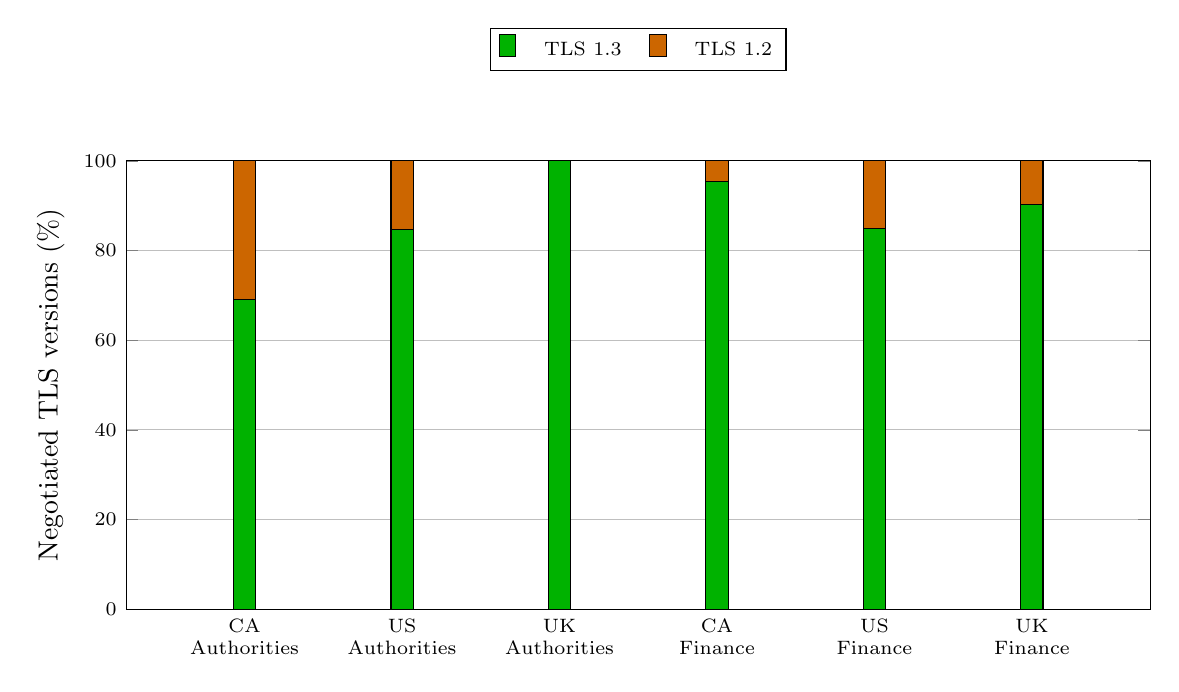
\begin{tikzpicture}
      \begin{axis}[
        ybar stacked,
        bar width=8pt,
        x=2cm,
        enlarge x limits=0.15,
        ymin=0, ymax=100,
        ylabel={Negotiated TLS versions (\%)},
        symbolic x coords={CA-Auth,US-Auth,UK-Auth,CA-Fin,US-Fin,UK-Fin},
        xtick=data,
        xticklabels={
          CA\\Authorities,
          US\\Authorities,
          UK\\Authorities,
          CA\\Finance,
          US\\Finance,
          UK\\Finance
        },
        xticklabel style={
          align=center,
          font=\scriptsize,
          text width=1.6cm
        },
        tick label style={font=\scriptsize},
        ymajorgrids=true,
        legend style={
          at={(0.5,1.20)},
          anchor=south,
          legend columns=3,
          column sep=8pt,
          font=\scriptsize,
        },
      ]

        \addplot[fill=green!70!black] coordinates {
          (CA-Auth, 69.1)
          (US-Auth, 84.6)
          (UK-Auth,100.0)
          (CA-Fin, 95.4)
          (US-Fin, 84.9)
          (UK-Fin, 90.2)
        };

        \addplot[fill=orange!80!black] coordinates {
          (CA-Auth, 30.9)
          (US-Auth, 15.4)
          (UK-Auth,  0.0)
          (CA-Fin,  4.6)
          (US-Fin, 15.1)
          (UK-Fin,  9.8)
        };

        \legend{TLS 1.3, TLS 1.2}
      \end{axis}
    \end{tikzpicture}}

    \caption{Stacked bar chart of negotiated TLS versions for authority and finance websites by country.}
    \label{fig:tls_stacked_auth_fin}
  \end{adjustbox}
\end{figure}

\subsubsection{Vulnerability disclosure (\texttt{security.txt})}
Table~\ref{tab:securitytxt_summary} presents adoption of RFC~9116 \texttt{security.txt}. Among Canadian authority origins, only 1.1\% (4/375) published a \texttt{security.txt} file. 
All four included contact and expiration fields, but only 25\% had unexpired \texttt{Expires} values at scan time. 
US Authorities showed higher adoption at 3.5\% (13/373), with most including \texttt{Expires} and a large fraction maintaining valid expiration dates. 
Overall, standardized disclosure signaling was rare across all measured populations. 


% table for security.txt summary
\begin{table}[t]
  \caption{Security.txt adoption and field completeness by dataset.}
  \label{tab:securitytxt_summary}
  \centering
  \scriptsize
  \setlength{\tabcolsep}{2.2pt} 
  \renewcommand{\arraystretch}{1.15}

  \begin{adjustbox}{max width=\columnwidth}
  % \resizebox{\columnwidth}{!}{%
  \csvreader[
    tabular=lr rr ccc,
    table head=\toprule
      Dataset &
      $n$ orig. &
      \multicolumn{2}{c}{security.txt present} &
      Contact (\%) &
      Expires (\%) &
      Valid exp. (\%) \\
      \cmidrule(lr){3-4}
      & & Count & Share (\%) & & & \\\midrule,
    late after line=\\,
    late after last line=\\\bottomrule
  ]{../results/comparison/securitytxt/securitytxt_summary.csv}{%
    dataset_label=\Dataset,
    n_origins=\Norigins,
    n_with_securitytxt=\Nwith,
    pct_sites_with_securitytxt=\Psites,
    pct_with_contact_among_present=\Pcontact,
    pct_with_expires_among_present=\Pexpires,
    pct_valid_expires_among_expires=\Pvalid
  }{%
    \Dataset &
    \Norigins &
    \Nwith &
    \Psites &
    \Pcontact &
    \Pexpires &
    \Pvalid
  }%
  \end{adjustbox}
\end{table}

\subsubsection{Security headers \& cookies}
Table~\ref{tab:security_headers_presence} summarizes security response header adoption at final resolved endpoints. Across datasets, legacy hardening headers appear more common than modern policy controls, with comparatively weaker deployment of CSP \texttt{frame-ancestors} and \texttt{Permissions-Policy}. 


% table for security headers presence
\begin{table}[t]
  \caption{Security header adoption by dataset (percent of final URIs).}
  \label{tab:security_headers_presence}
  \centering
  \scriptsize
  \setlength{\tabcolsep}{2.2pt}
  \renewcommand{\arraystretch}{1.15}

  \begin{adjustbox}{max width=\columnwidth}
  % \resizebox{\columnwidth}{!}{%
  \csvreader[
    tabular=lccccc,
    table head=\toprule
      Dataset &
      \shortstack{Referrer\\Policy} &
      \shortstack{X-Content-Type\\Options} &
      \shortstack{X-Frame\\Options} &
      \shortstack{CSP\\frame-ancestors} &
      \shortstack{Permissions\\Policy} \\\midrule,
    late after line=\\,
    late after last line=\\\bottomrule
  ]{../results/comparison/headers/security_headers_presence.csv}{%
    dataset_label=\Dataset,
    pct_referrer_policy_present=\Pref,
    pct_x_content_type_options_present=\Pxcto,
    pct_x_frame_options_present=\Pxfo,
    pct_csp_frame_ancestors_present=\Pcsp,
    pct_permissions_policy_present=\Pperm
  }{%
    \Dataset & \Pref & \Pxcto & \Pxfo & \Pcsp & \Pperm
  }%
  \end{adjustbox}
  \end{table}

Cookie attributes are summarized in Table~\ref{tab:cookie_security_flags}. For Canadian authorities, 28.2\% of endpoints set cookies; among those, 63.5\% set \texttt{Secure}, 48.7\% set \texttt{HttpOnly}, and only 15.7\% set \texttt{SameSite}$\ge$Lax. 
Only 3.5\% of Canadian authority cookie-setting endpoints met the recommended/sufficient cookie profile used in our evaluation. 

  % table for cookie security flags
\begin{table}[t]
    \caption{Cookie security flag adoption by country and sector.}
    \label{tab:cookie_security_flags}
    \centering
    \scriptsize
    \setlength{\tabcolsep}{3pt}
    \renewcommand{\arraystretch}{1.15}
    
    \begin{adjustbox}{max width=\columnwidth}
    % \resizebox{\columnwidth}{!}{%
    \csvreader[
      tabular=lllrrr,
      table head=\toprule
        Dataset &
        Sites w/ cookies (\%) &
        Secure flag (\%) &
        HttpOnly flag (\%) &
        SameSite$\ge$Lax (\%) &
        Rec./Suff. (\%) \\\midrule,
      late after line=\\,
      late after last line=\\\bottomrule
    ]{../results/comparison/headers/cookie_security_flags_summary.csv}{%
      dataset_label=\Dataset,
      pct_sites_with_cookies=\Pcookies,
      pct_secure_among_cookie_sites=\Psecure,
      pct_httponly_among_cookie_sites=\Phttp,
      pct_samesite_ge_lax_among_cookie_sites=\Psame,
      pct_rec_suff_among_cookie_sites=\Prec
    }{%
      \Dataset & \Pcookies & \Psecure & \Phttp & \Psame & \Prec
    }%
    \end{adjustbox}
  \end{table}

\subsubsection{Information leakage}
Technology-revealing response headers remain prevalent (Table~\ref{tab:revealing_headers_summary}). For Canadian authority origins, 94.4\% exposed at least one such header and 10.8\% exposed three or more. 
Error-response leakage is summarized in Table~\ref{tab:error_leaks_summary}. In Canadian authorities, 47.2\% of origins exhibited technology leakage in error responses and 10.7\% disclosed explicit version information. 
Comparable rates were observed in US and UK authorities, indicating that information disclosure through response metadata and default error handling remains a cross-jurisdiction issue. 


  % table for revealing headers summary
    \begin{table}[t]
      \caption{Distribution of technology-revealing headers by dataset.}
      \label{tab:revealing_headers_summary}
      \centering
      \scriptsize
      \setlength{\tabcolsep}{3pt}
      \renewcommand{\arraystretch}{1.15}
    
      \begin{adjustbox}{max width=\columnwidth}
      % \resizebox{\columnwidth}{!}{%
      \csvreader[
        tabular=lrrrrrc,
        table head=\toprule
          Dataset &
          $n$ sites &
          \multicolumn{4}{c}{$n$ revealing headers (\%)} &
          Any (\%) \\
          \cmidrule(lr){3-6}
          & & 0 & 1 & 2 & 3+ & \\\midrule,
        late after line=\\,
        late after last line=\\\bottomrule
      ]{../results/comparison/headers/revealing_headers_summary.csv}{%
        dataset_label=\Dataset,
        n_sites=\Nsites,
        pct_revealing_0=\Pzero,
        pct_revealing_1=\Pone,
        pct_revealing_2=\Ptwo,
        pct_revealing_3_plus=\Pthree,
        pct_with_any_revealing=\Pany
      }{%
        \Dataset &
        \Nsites &
        \Pzero &
        \Pone &
        \Ptwo &
        \Pthree &
        \Pany
      }%
      \end{adjustbox}
    \end{table}
    

    % table for error leaks summary
    % Error Leaks Summary Table
    \begin{table}[t]
      \caption{Information leakage in HTTP error responses by dataset.}
      \label{tab:error_leaks_summary}
      \centering
      \scriptsize
      \setlength{\tabcolsep}{4pt}
      \renewcommand{\arraystretch}{1.15}
      
      \begin{adjustbox}{max width=\columnwidth}
      % \resizebox{\columnwidth}{!}{%
      \csvreader[
        tabular=lrrr,
        table head=\toprule
          Dataset &
          $n$ origins &
          Any tech leak (\%) &
          Version leak (\%) \\\midrule,
        late after line=\\,
        late after last line=\\\bottomrule
      ]{../results/comparison/error_leaks/error_leaks_summary.csv}{%
        dataset_label=\Dataset,
        n_scanned_origins=\Norigins,
        pct_any_tech_leak=\Ptech,
        pct_version_leak=\Pversion
      }{%
        \Dataset & \Norigins & \Ptech & \Pversion
      }%
      \end{adjustbox}
    \end{table}

% NOTE: Here I hardcoded the number of unique entries from the final + input origins
% for each sector. Reason being is I forgot to record it in the data,
% and the following tables use the unique number, not the sum (input + final).
% I felt like it was potentially misleading/confusing to the reader not
% show these numbers explicitly. The reader would likely expect the sum.
% \begin{table}[t]
%   \caption{Redirect resolution summary (inputs mapped to measured endpoints).}
%   \label{tab:redirect_summary}
%   \centering
%   \scriptsize
%   \setlength{\tabcolsep}{3pt}
%   \renewcommand{\arraystretch}{1.15}
%   \begin{adjustbox}{max width=\columnwidth}
%   % \resizebox{\columnwidth}{!}{%
%   \csvreader[
%     tabular=lrrrrr,
%     table head=\toprule
%       Dataset &
%       \multicolumn{2}{c}{\emph{n} URIs} &
%       \multicolumn{2}{c}{\emph{n} Origins} &
%       Final 2xx (\%) \\
%       \cmidrule(lr){2-3}\cmidrule(lr){4-5}
%        & Input & Final & Input & Unique & \\
%       \midrule,
%     late after line=\\,
%     late after last line=\\\bottomrule
%   ]{../results/comparison/redirects/redirects_summary.csv}{%
%     dataset_label=\Dataset,
%     n_input_uris=\Nuris,
%     n_final_uris=\Nfinal,
%     n_input_origins=\NorigIn,
%     pct_final_2xx=\Ptwo
%   }{%
%     \Dataset &
%     \Nuris &
%     \Nfinal &
%     \NorigIn &
%     \ifnum\pdfstrcmp{\Dataset}{CA Authorities}=0 375\fi%
%     \ifnum\pdfstrcmp{\Dataset}{CA Education}=0 103\fi%
%     \ifnum\pdfstrcmp{\Dataset}{CA Finance}=0 157\fi%
%     \ifnum\pdfstrcmp{\Dataset}{CA Energy}=0 188\fi%
%     \ifnum\pdfstrcmp{\Dataset}{US Authorities}=0 373\fi%
%     \ifnum\pdfstrcmp{\Dataset}{US Education}=0 53\fi%
%     \ifnum\pdfstrcmp{\Dataset}{US Finance}=0 107\fi%
%     \ifnum\pdfstrcmp{\Dataset}{US Energy}=0 141\fi%
%     \ifnum\pdfstrcmp{\Dataset}{UK Authorities}=0 4\fi%
%     \ifnum\pdfstrcmp{\Dataset}{UK Education}=0 447\fi%
%     \ifnum\pdfstrcmp{\Dataset}{UK Finance}=0 165\fi%
%     &
%     \Ptwo
%   }%
%   \end{adjustbox}
%   \end{table}

  

\section{Discussion}\label{sec:discussion}
This study benchmarked transport and browser-enforced web security controls across Canadian public-sector and critical-sector websites, with comparative measurements against the United States and United Kingdom. Overall, baseline transport encryption is widely deployed, but stronger controls are inconsistently implemented in Canadian authorities, and application-layer hardening remains sparse across all jurisdictions.

\subsection{What the results imply}
\paragraph{Transport security is common, but enforcement is uneven}
Most Canadian authority origins are HTTPS-reachable and many upgrade HTTP to HTTPS, suggesting that encrypted transport is now the default for a substantial portion of the public-sector surface. However, a non-trivial fraction still serves HTTP without upgrade, and HSTS is not consistently deployed. Since HSTS (RFC~6797) is a browser-enforced mechanism that prevents downgrade and first-visit stripping attacks, gaps here represent avoidable exposure that can often be fixed at the edge (e.g., reverse proxy/CDN)~\cite{rfc6797,mdn_sts_header}.

\paragraph{Modern configurations lag behind policy-driven peers}
Canadian authorities negotiate TLS~1.3 less frequently than the comparison authority datasets, and HSTS adoption is lower and less often configured strongly (e.g., long max-age with \texttt{includeSubDomains}). These differences are consistent with Canada relying primarily on guidance (CCCS) rather than enforceable directives, while the U.S.\ and U.K.\ have centralized policy and operational mechanisms that more directly drive compliance~\cite{cccs-itsp-40062,cccs-itsm-60005,omb-m-15-13,cisa_bod_18_01,uk-using-https-service-manual}.

\paragraph{Browser-enforced hardening remains a major gap}
Across datasets, security response headers and cookie attributes are not deployed with the same consistency as transport controls. This matters because modern web attacks frequently exploit browser behaviors (e.g., framing, referrer leakage, cross-site requests, content injection) that are mitigated by policy headers and robust cookie settings~\cite{owasp_http_security_response_headers,mdn_secure_cookie_configuration}. In practice, many of these controls can be standardized through platform templates, central gateways, or shared middleware.

\paragraph{Low disclosure readiness + high leakage is a problematic combination}
Adoption of RFC~9116 \texttt{security.txt} is near-zero across all populations measured, including Canadian authorities. Yet technology fingerprinting opportunities remain common through response headers and error handling. This combination both lowers the cost of reconnaissance and raises the friction for responsible reporting, increasing the likelihood that vulnerabilities persist longer than necessary~\cite{rfc9116,cwe_209,owasp_secure_headers_project}.

% \subsection{Actionable takeaways}
% The gaps we observe largely reflect \emph{configuration} rather than exotic engineering changes. Many improvements are low-effort and can be deployed without application rewrites:
% (i) enforce HTTPS-only with strong HSTS at all public origins;
% (ii) standardize modern TLS defaults and retire legacy protocol support;
% (iii) adopt a minimal baseline of security headers (e.g., \texttt{Referrer-Policy}, anti-framing controls via CSP \texttt{frame-ancestors}, \texttt{nosniff}, and \texttt{Permissions-Policy});
% (iv) harden cookies by default (\texttt{Secure}, \texttt{HttpOnly}, and \texttt{SameSite} where feasible); and
% (v) publish and maintain \texttt{security.txt} for all internet-accessible systems~\cite{rfc9116,cisa_securitytxt_simple_file_big_value}.
% Given the observed cross-jurisdiction differences, translating Canadian guidance into more uniform operational requirements (or compliance frameworks) may substantially reduce variance in adoption~\cite{cccs-itsp-40062,cccs-itsm-60005}.

\section{Conclusion}
Canadian public-sector websites generally exhibit strong baseline encryption, but stronger transport enforcement and modern browser-side controls are inconsistently deployed, especially among authority sites. Standardized vulnerability disclosure remains rare, while information leakage via response metadata and error handling is common. 
Our results motivate configuration-focused remediation (e.g., strong HSTS, modern TLS defaults, baseline security headers, and hardened cookies) and continued benchmarking to track progress and support operational and policy improvements.

This study has limitations. Measurements reflect an external vantage point under strict ethical rate limits; ``unreachable'' outcomes may stem from
 bot mitigation/WAF behavior rather than true downtime. Header and cookie evaluations were performed
  on resolved landing pages and may differ on authenticated or transactional paths. 
  Measurements also reflect a snapshot rather than longitudinal behavior. 
  Since web configurations can change due to routine updates, outages, or temporary infrastructure conditions, the reported rates
   should be interpreted as observations from the measurement window rather than permanent properties. 
   In addition, some comparison datasets are smaller than others, particularly certain UK subsets. 
   This limits the strength of direct cross-dataset comparisons involving those subsets.
  Furthermore, our \texttt{security.txt} discovery did not follow cross-origin redirects, potentially undercounting
   centralized deployments. Finally, we measure control adoption rather than exploitability: missing controls
    increase exposure but do not imply a specific vulnerability.

Future work includes longitudinal re-scans to quantify change over time, broader endpoint coverage (e.g., login and high-value workflows), and dependency/third-party resource analysis to better understand supply-chain exposure and external hosting reliance~\cite{hsiao2019cyberautonomy}.

% \section{Discussion}\label{sec:discussion}


% This study measured the adoption of transport and browser-enforced web security controls across Canadian public-sector and
% critical-sector sites, with cross-jurisdiction comparisons to the United States and United Kingdom.
% Overall, baseline transport security is widely deployed across most datasets, but
% adoption is uneven in Canadian authorities and stronger controls are not consistently enforced.
% Across sectors, modern browser-side hardening remains sparse relative to transport-level adoption. 
% Furthermore, technology disclosure through response metadata and error handling remains common,
% indicating that low-effort fingerprinting opportunities still persist even where HTTPS is present.

    
% First, the results show that transport protections are common but not ubiquitous. 
% Most measured origins are HTTPS-reachable and the majority of HTTP-accessible services upgrade users to HTTPS (Table~\ref{tab:https_connectivity}), 
% indicating that HTTPS is now the default for much of the Canadian web. Within Canada, non-authority datasets typically
% show stronger transport reachability behavior than authorities (Table~\ref{tab:https_connectivity}).  
% Moreover, in all datasets most services upgrade users via redirection (Table~\ref{tab:https_connectivity}),
% yet a substantial portion of Canadian authority sites still serve HTTP without upgrading (6.43\%). Likewise, Canadian
% authorities remain the lowest-performing Canadian sector on TLS~1.3 compatability and default negotiation (Fig.~\ref{fig:tls_stacked_auth_fin}). 
% Accross jurisdictions, TLS configurations remained quite strong, although a considerable portion still advertises legacy TLS protocol support (Table~\ref{tab:tls_summary}). 
% Most sites in all jurisdictions naturally negotiated the widely recommended TLS~1.3, with 0\% of sites negotiating legacy TLS.

% Browser-enforced controls show the largest adoption gaps. At the application layer, Canadian authority endpoints more frequently implement legacy hardening
%  headers such as \texttt{X-Frame-Options} and \texttt{X-Content-Type-Options} than modern policy controls, with notably weaker adoption
%  of CSP \texttt{frame-ancestors} and \texttt{Permissions-Policy} (Table~\ref{tab:security_headers_presence}). HSTS adoption among Canadian
% authority sites is on the lower-end, with over 40\% of sites not supporting HSTS, and of those only 27.43\% appear on the preload list (Table~\ref{tab:https_hsts_quality}).
% Accross all datsets, the fraction of cookies that meet recommended or sufficient attribute profiles was found to be extremely small
%  (only 3.5\% for CA authorities) (Table~\ref{tab:cookie_security_flags}).

% Similarlities are present in both information leakage and vulnerability disclosure. A substantial fraction of all datasets contain revealing headers and
% leak technology information in error responses. Additionally, a non-trivial fraction leak version information, including nearly 50\% of the Canadian authority sites evaluated (Table~\ref{tab:revealing_headers_summary} and Table~\ref{tab:error_leaks_summary}). 
% Notably, near-zero origins hosted a \texttt{security.txt} file in all datasets, despite the prevalence of information leakage. Regarding Canadian authorities, 
% only 4 of 375 origins were found to host a \texttt{security.txt} file, of which 75\% contained an expired Expires field (Table~\ref{tab:securitytxt_summary}). 
% This combination is especially consequential because it lowers the cost of reconnaissance while simultaneously reducing the likelihood that external researchers 
% can report issues through a standardized channel.


% \subsection{Conclusion}

% Importantly, these are not exotic mitigations. Many are low-effort, configuration-driven controls 
% that can be deployed at the edge (CDN/WAF/reverse proxy) without application rewrites. The results suggest that the gaps found in 
% Canadian web security is not a lack of
% technical capability, but inconsistent adherence to existing guidance. The CCCS publishes comprehensive, 
% and pragmatic recommendations for securing both the transport and application layer of HTTP. However, the
% contrast with US federal practice is apparent. Our cross-country results 
% reflect the difference in governance models found in the UK and US. The results illustrate a higher and more uniform 
% adoption of the same controls in the US and UK, despite them being recommended in Canada. Web configuration and development 
% is complex and web development remains one of the most rapidly changing areas of IT. Converting recommendations 
% into consistently applied practice would reduce exposure to common attacks and better
% honour the trust that Canadians place in online public services.


% \subsection{Limitations}

% This measurement study has several limitations. First, results reflect the scanner’s network vantage point and
% strict ethical rate limits. Some ``unreachable'' outcomes may reflect bot mitigation or WAF policies rather than
% service unavailability. However, from an external user perspective, aggressive filtering can still function as a
% practical availability barrier, and therefore remains relevant to posture. Second, our header and cookie analysis
% was performed on landing-page responses. Some sites may apply stricter controls on authenticated or transactional
% paths. Third, \texttt{security.txt} discovery did not follow cross-origin redirects, which may undercount sites
% that host disclosure policy on centralized origins. Finally, this study evaluates security control adoption rather
% than exploitability: absence of a control indicates increased risk exposure, but not necessarily the presence of a
% specific vulnerability.

% \subsection{Future Work}

% Future work should extend this benchmarking methodology in three directions. First, longitudinal scans would
% quantify change over time and assess whether policy interventions measurably improve posture. 
% Second, expanding endpoint coverage beyond landing pages (e.g., authentication and high-value workflows) would better capture how
% controls vary across application surfaces. Third, deeper dependency analysis could quantify third-party resource
% exposure and content supply-chain risk, complementing prior findings that government sites often rely on external
% infrastructure~\cite{hsiao2019cyberautonomy}. Together, these extensions would enable continuous measurement of
% Canada’s public-sector web security maturity, supporting both operational remediation and evidence-based policy.

\section*{Acknowledgment}

This work was supported by the CSA Group Undergraduate Research Scholarship. We thank the CSA Group staff for their guidance in developing recommendations to formalize web security standards for Canadian public-sector domains.
% \section*{References}

\bibliographystyle{IEEEtran}
\bibliography{main}

% Please number citations consecutively within brackets~\cite{b1}. The 
% sentence punctuation follows the bracket~\cite{b2}. Refer simply to the reference 
% number, as in~\cite{b3}---do not use ``Ref.~\cite{b3}'' or ``reference~\cite{b3}'' except at 
% the beginning of a sentence: ``Reference~\cite{b3} was the first $\ldots$''

% Number footnotes separately in superscripts. Place the actual footnote at 
% the bottom of the column in which it was cited. Do not put footnotes in the 
% abstract or reference list. Use letters for table footnotes.

% Unless there are six authors or more give all authors' names; do not use 
% ``et al.''. Papers that have not been published, even if they have been 
% submitted for publication, should be cited as ``unpublished''~\cite{b4}. Papers 
% that have been accepted for publication should be cited as ``in press''~\cite{b5}. 
% Capitalize only the first word in a paper title, except for proper nouns and 
% element symbols.

% For papers published in translation journals, please give the English 
% citation first, followed by the original foreign-language citation~\cite{b6}.

% \begin{thebibliography}{00}
% \bibitem{b1} G. Eason, B. Noble, and I. N. Sneddon, ``On certain integrals of Lipschitz-Hankel type involving products of Bessel functions,'' Phil. Trans. Roy. Soc. London, vol. A247, pp. 529--551, April 1955.
% \bibitem{b2} J. Clerk Maxwell, A Treatise on Electricity and Magnetism, 3rd ed., vol. 2. Oxford: Clarendon, 1892, pp.68--73.
% \bibitem{b3} I. S. Jacobs and C. P. Bean, ``Fine particles, thin films and exchange anisotropy,'' in Magnetism, vol. III, G. T. Rado and H. Suhl, Eds. New York: Academic, 1963, pp. 271--350.
% \bibitem{b4} K. Elissa, ``Title of paper if known,'' unpublished.
% \bibitem{b5} R. Nicole, ``Title of paper with only first word capitalized,'' J. Name Stand. Abbrev., in press.
% \bibitem{b6} Y. Yorozu, M. Hirano, K. Oka, and Y. Tagawa, ``Electron spectroscopy studies on magneto-optical media and plastic substrate interface,'' IEEE Transl. J. Magn. Japan, vol. 2, pp. 740--741, August 1987 [Digests 9th Annual Conf. Magnetics Japan, p. 301, 1982].
% \bibitem{b7} M. Young, The Technical Writer's Handbook. Mill Valley, CA: University Science, 1989.
% \end{thebibliography}
% \vspace{12pt}
% \color{red}
% IEEE conference templates contain guidance text for composing and formatting conference papers. Please ensure that all template text is removed from your conference paper prior to submission to the conference. Failure to remove the template text from your paper may result in your paper not being published.

\end{document}
